\section{Les mémoires}



%%%%%%%%%%%%%%%%%%%%%%%%%%%%%%%%%%%%%%%%%%%%%%%%%%%%%%%%%%%%%%%%%%%
\subsection{La mémoire}
%%%%%%%%%%%%%%%%%%%%%%%%%%%%%%%%%%%%%%%%%%%%%%%%%%%%%%%%%%%%%%%%%%%









%%%%%%%%%%%%%%%%%%%%%%%%%%%%%%%%%%%%%%%%%%%%%%%%%%%%%%%%%%%%%%%%%%%
\subsection{Les technologies mémoires}
%%%%%%%%%%%%%%%%%%%%%%%%%%%%%%%%%%%%%%%%%%%%%%%%%%%%%%%%%%%%%%%%%%%
















%%%%%%%%%%%%%%%%%%%%%%%%%%%%%%%%%%%%%%%%%%%%%%%%%%%%%%%%%%%%%%%%%%%
\section{Hiérarchie mémoire}
%%%%%%%%%%%%%%%%%%%%%%%%%%%%%%%%%%%%%%%%%%%%%%%%%%%%%%%%%%%%%%%%%%%

\begin{fancyquotes}
Idéalement, on souhaiterait disposer d'une capacité de mémoire indéfiniment grande, de sorte qu'un agrégat particulier de 40 chiffres binaires, ou mot (cf. 2.3), soit immédiatement disponible, c'est-à-dire dans un temps légèrement ou considérablement plus court que le temps de fonctionnement d'un multiplicateur électronique rapide. On peut supposer que cela est pratique au niveau d'environ 100 m sec. Par conséquent, le temps de disponibilité d'un mot dans la mémoire doit être de 5 à 50 ms. Il est également souhaitable que les mots puissent être remplacés par de nouveaux mots à peu près au même rythme. Il ne semble pas physiquement possible d'atteindre une telle capacité. Nous sommes donc obligés de reconnaître la possibilité de construire une hiérarchie de mémoires, chacune d'entre elles ayant une plus grande capacité que la précédente mais moins rapidement accessible.\\
Traduit de \cite{burks1946preliminary}.

\end{fancyquotes}


\subsection{Motivations}
%%%%%%%%%%%%%%%%%%%%%%%%%%%%%%%%%%%%%%%%%%%%%%%%%%%%%%%%%%%%%%%%%%%


Dès 1946, les architectes des processeurs avaient anticipé que les applications seraient demandeuses de mémoires très performantes. A cause de la forte évolution du processeur, l'écart avec la performance des mémoires s'est creusé au fil des années (voir \autoref{pic:cpuvsmemory}). L'incapacité du processeur d'accéder suffisamment rapidement à la mémoire est inhérent à l'architecture actuelle des processeurs qui partage le même bus pour accéder aux instructions et aux données stockées en mémoire. Ce \textit{goulot d'étranglement} ou \textit{bottleneck}, a été nommé d'après l'un des architectes de l'architecture: le \textit{bottleneck Von Neumann}.


\begin{figure}
    \center
    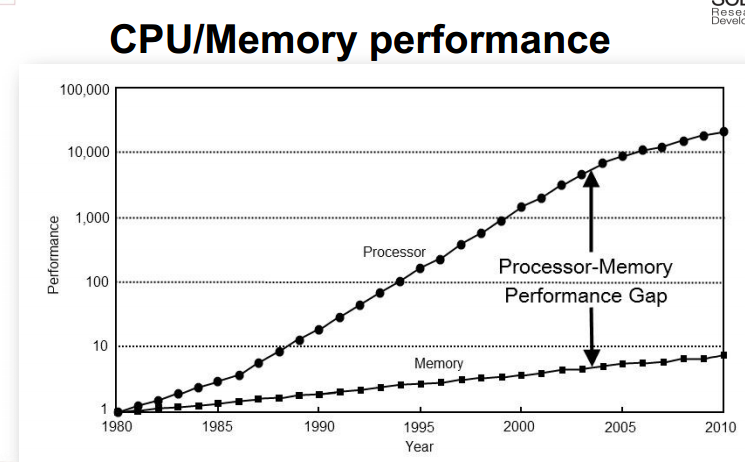
\includegraphics[width=10cm]{images/cpu_vs_memory.png}
    \caption{\label{pic:cpuvsmemory} Progression de la performance des processeurs et des mémoires. Les processeurs ont vu leur performance évoluer de 50\% chaque année, contre 7\% pour les mémoires. L'écart de performance entre les deux matériels s'est creusé de 50\%  chaque année depuis les années 2000 (graphique extrait de \cite{AliSalehi2012}).}
\end{figure}

La réponse naïve à ce problème est de construire de grande mémoire à partir de SRAM, très performante et qui consomme peu d'énergie. Cependant, des contraintes économiques et technique sont à prendre en compte et rendent impossible cette solution. La mémoire SRAM est très cher à produire et nécessite l'utilisation de six transistors pour fonctionner, empêchant la construction de modules denses. Les constructeurs de processeurs ont dû élaborer une solution en prenant en compte la vitesse, la densité et le coût de chacune des technologies mémoires. Au plus une mémoire est rapide, au plus sont coût est élevé. Au plus la densité est élevée, plus le prix par bit stocké est réduit. Au plus la densité est élevé, au plus le temps d'accès est élevé. 






\subsection{Hiérarchie mémoire sur les processeurs récents}
%%%%%%%%%%%%%%%%%%%%%%%%%%%%%%%%%%%%%%%%%%%%%%%%%%%%%%%%%%%%%%%%%%%

La hiérarchie mémoire est la réponse économique et technique apportée aux contraintes évoquées ci dessus. Elle consiste en l'utilisation de différents modules mémoires de tailles, de technologies et de performances différentes. Son objectif peut être résumé à trois points: réduire le coût par bit stocké, augmenter la capacité de la mémoire la plus rapide, améliorer le temps d'accès aux données. La solution est de placer au plus proche du processeur des mémoires très rapide pouvant répondre instantanément aux accès mémoire. Au plus on s'éloigne des unités de calcul, au plus la latence d'accès aux modules mémoires augmente, mais au plus leur prix diminue rendant possible l'utilisation de module de plus grande capacité.


Les différents niveaux de mémoire peuvent être imbriqués, une donnée qui se trouve dans le premier niveau sera aussi stockée dans les modules de niveaux supérieurs.

Lorsque le processeur souhaite accéder à une donnée, il vérifie qu'elle se trouve dans son premier niveau de mémoire et, si ce n'est pas le cas, remonte la hiérarchie jusqu'à la trouver. La performance des applications varie fortement si les données nécessaires sont présentes ou non dans les mémoires proches du processeur. Les programmes doivent essayer de profiter du concept de localité présenté dans la section \autoref{sec:localite}.
\begin{figure}
    \center
    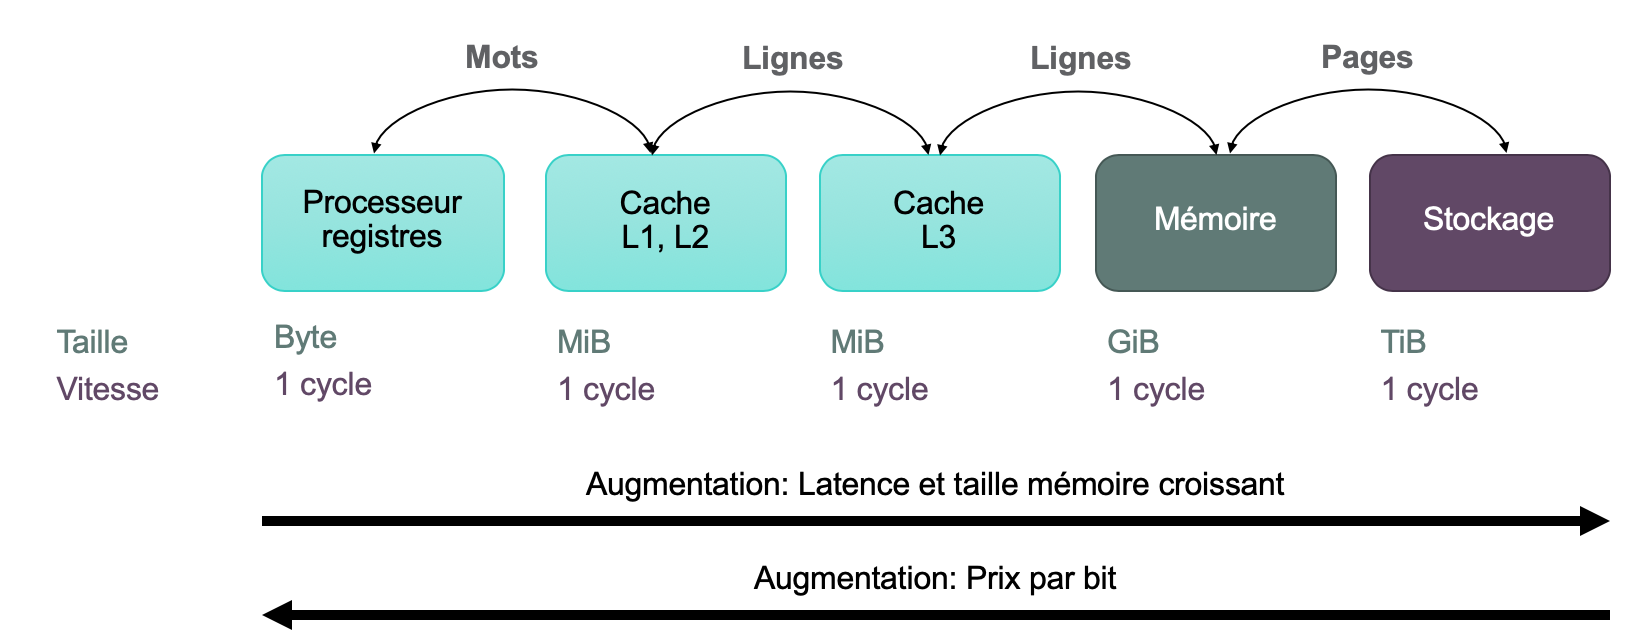
\includegraphics[width=14cm]{images/memory_hierarchy.png}
    \caption{\label{pic:cpuvsmemory} Hiérarchie mémoire}
\end{figure}





\subsection{Communication entre les différents niveaux}
%%%%%%%%%%%%%%%%%%%%%%%%%%%%%%%%%%%%%%%%%%%%%%%%%%%%%%%%%%%%%%%%%%%
Pour communiquer entre les différents niveaux de la hierarchie les données sont transmises par bloc de données de tailles différentes. L'avantage de tranférer les données par bloc et non une par une est d'amlélirer la performance des codes en tirant parti du principe de localité spatiale (voir \autoref{sec:localite}).
Pour accéder à un mot, le processeur a besoin que celle ci se trouve dans le niveau de cache L1. Lorsqu'elle si trouve, le processeur peut charger un mot directement dans ces registres pour y effectuer les opérations nécessaires. C'est la granularité de transfert la plus petite dans un ordinateur. 

Entre les différents niveaux de caches et entre le cache et la mémoire les données sont transférées par blocs appellées \textit{lignes de cache} ou \textit{cache line}. La ligne de cache contient une copie des données de la mémoire, un tag contenant des informations sur l'adresse mémoire du bloc de donnée et un \textit{flag} contenant des informations sur la validité de la ligne (voir \autoref{pic:cacheline}). La taille d'une ligne de cache peut varier d'une architecture à l'autre mais il est courant d'utiliser des tailles de 32, 64 ou 128 bytes. Une ligne de cache d'un processeur Intel récent mesure 64 bytes. Elle contient ainsi entre 8 et 16 éléments en double précision. 

\begin{figure}
    \center
    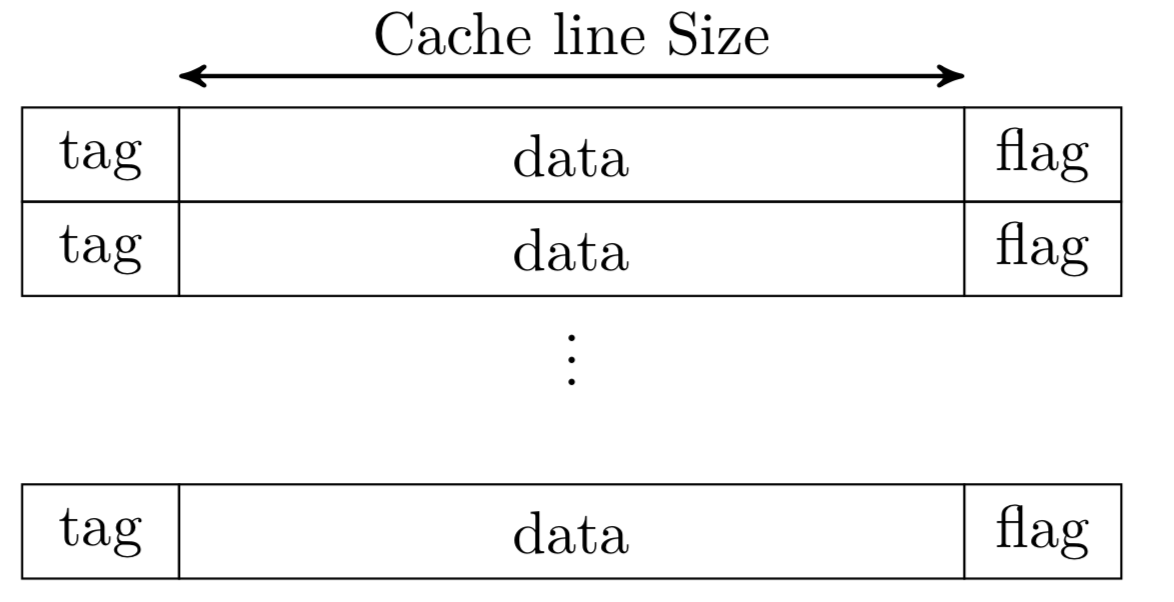
\includegraphics[width=8cm]{images/cacheline_def.png}
    \caption{\label{pic:cacheline} Représentation d'une ligne de cache.}
\end{figure}


Entre la mémoire, les blocs de données transférés sont de la taille d'une page (voir \autoref{sec:page}) qui mesure généralement entre 4 KiB et 2 MiB.



\subsection{Registres}
%%%%%%%%%%%%%%%%%%%%%%%%%%%%%%%%%%%%%%%%%%%%%%%%%%%%%%%%%%%%%%%%%%%
Les registres du processeurs sont situés au plus proche des unités de calculs. Pour permettre un accès rapide, 1 cycle, ils sont réalisés en SRAM. On compte entre x et y registres sur les processeurs récents. Leur taille est variable en fonction des instructions exécutables par les unités logiques arithmétiques. Par exemple, un processeur pouvant exécuter des instructions vectorielles AVX-512, possède des registres de 512 bits (registre \textit{ZMM}). Il existe différents types de registres, certains sont utilisés pour stocker des données et des résultats intermédiaires, tandis que d’autres ont une signification précise. Le registre de pointeurs de piles stocke l’adresse de la première adresse mémoire responsable de l’instruction actuellement exécutée et permettent de réaliser des appels et des retours de fonctions. Les registres des drapeaux (Flag Register) stockent des informations nécessaire à l’éxécution d’instructions. Par exmple, lorsqu’une retenue est générée par un calcul, ou qu’un branchement conditionnelle a été évalué à vrai. Les processeurs récents dupliquent certains registres pour pouvoir utiliser des techniques de renommage \cite{moudgill1993register} et d'exécution spéculative \cite{chou2004efficient}. Lors de l'exécution d'une instruction nécessitant plusieurs cycles, le processeur, si aucune dépendance n'est détectée, commence à exécuter les instructions suivantes sans attendre le résultat de la première instruction.



%%%%%%%%%%%%%%%%%%%%%%%%%%%%%%%%%%%%%%%%%%%%%%%%%%%%%%%%%%%%%%%%%%%
%%%%%%%%%%%%%%%%%%%%%%%%%%%%%%%%%%%%%%%%%%%%%%%%%%%%%%%%%%%%%%%%%%%
\subsection{Caches}
%%%%%%%%%%%%%%%%%%%%%%%%%%%%%%%%%%%%%%%%%%%%%%%%%%%%%%%%%%%%%%%%%%%
%%%%%%%%%%%%%%%%%%%%%%%%%%%%%%%%%%%%%%%%%%%%%%%%%%%%%%%%%%%%%%%%%%%
C’est en 1965 que les premières mémoires caches sont présentées sous le nom de \textit{slave memory} \cite{wilkes1965slave}. Leur temps d’accès est de 4 à 20 fois plus rapide que celui de la mémoire principale servant alors de mémoire tampon. 

Lorsque le processeur doit accéder à une donnée, il commence par la chercher dans le premier niveau de cache, si elle si trouve, son temps d'accés est très rapide (évenement \textit{cache hit}). Si ce n’est pas le cas (évenement \textit{chache miss}), il réalise alors une copie de la zone mémoire la contenant dans le cache. La zone mémoire copié est appelé \textit{ligne de cache}. Si par la suite, cette donnée ou une donnée appartement à la même ligne de cache devait être à nouveau accédée, leur temps d’accès serait alors drastiquement réduit. Ce mécanisme est transparent pour l’utilisateur, bien que pour des questions de performances il doive être conscient de son existence (voir \autoref{sec:localite}). 

La taille de chaque niveau de cache varie pour les raisons expliquées en introduction de cette partie. A cela vient s'ajouter la notion de performance qui est lié à la tache du cache. Un cache de grande capacité aura plus de chance de contenir la donnée dont le processeur à besoin, améliorant ainsi la performance moyenne du programme. Cependant, un cache plus grand nécessite plus de comparaison pour vérifier si une donnée si trouve ou non. Pour allier les avantages et contourner les inconvénient, les processeurs utilisent non pas un, mais plusieurs niveaux de caches de tailles différentes.
Le premier niveau de cache est généralement séparé en deux zone mémoire: l'une contenant les instructions et l'autre les données. C'est le seul niveau de la hiérarchie qui stocke différemment les données et les instructions. Sur les processeurs récents, le premier et le deuxième niveau de cache est privé à chaque coeur. Un troisième, et parfois un quatrième niveau de cache est partagé entre les différents coeurs du processeur. La \autoref{pic:cache_hierarchy} représente une telle architecture pour un processeur à 4 coeurs.

\begin{figure}
    \center
    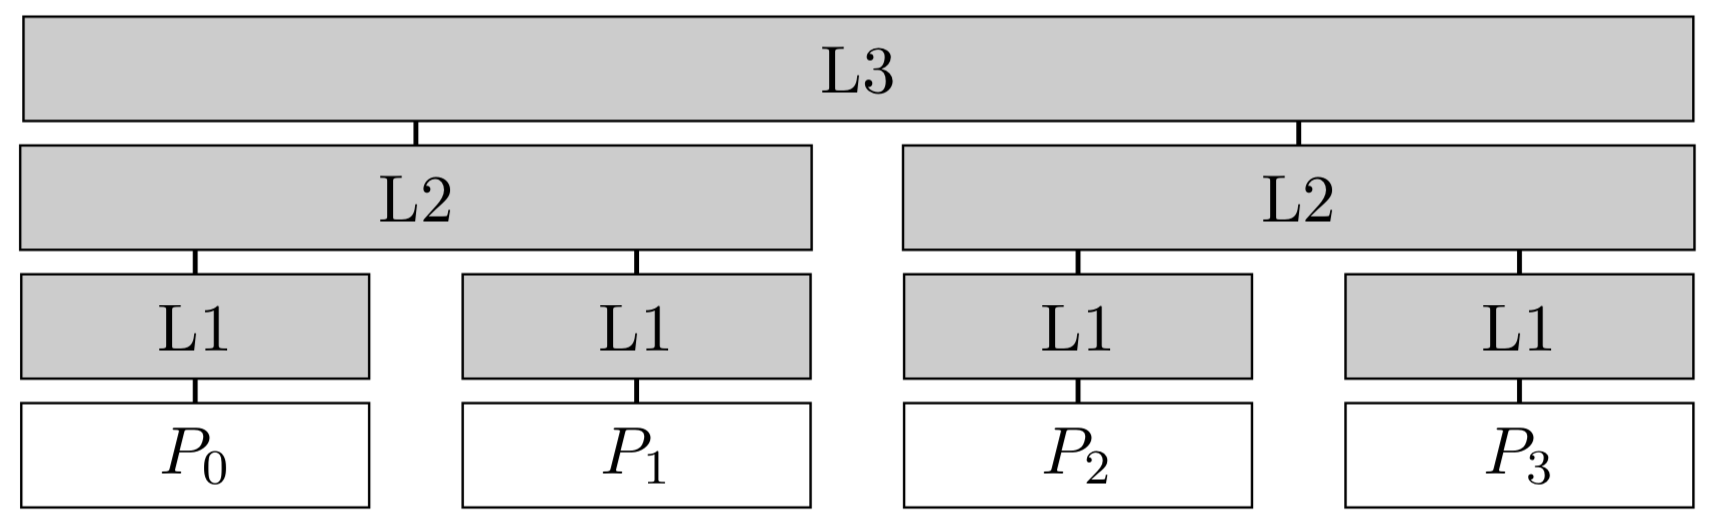
\includegraphics[width=8cm]{images/cache_hierarchy.png}
    \caption{\label{pic:cache_hierarchy} Organisation d'une hiérarchie de cache à trois niveau sur un processeur à 4 coeurs (source \cite{putigny2014benchmark}).}
\end{figure}



\subsubsection{Politique de placement: associativité}
%%%%%%%%%%%%%%%%%%%%%%%%%%%%%%%%%%%%%%%%%%%%%%%%%%%%%%%%%%%%%%%%%%%
La performance d'un cache ne vient pas seulement de la technologie utilisée pour sa construction. En effet, lorsqu'une donnée est accédé, le cache doit vérifier si la donnée est présente ou non dans le niveau de cache demandé. Il faut que l'algorithme de comparaison de permettant de la trouver soit le plus rapide possible. Pour cela, les architectes utilisent généralement une fonction de \textit{hash} permettant d'attribuer un emplacement dans le cache en fonction de l'adresse de la \textit{cache line}. Si la \textit{cache line} ne s'y trouve pas, c'est quelle n'est pas présente dans ce niveau de cache.
Les trois politiques de placement les plus utilisées sont: le mappage  \textit{direct }, le mappage \textit{fully associative} et le mappage \textit{set assiociative} (voir \autoref{pic:cache_associativite}).


\begin{figure}
    \center
    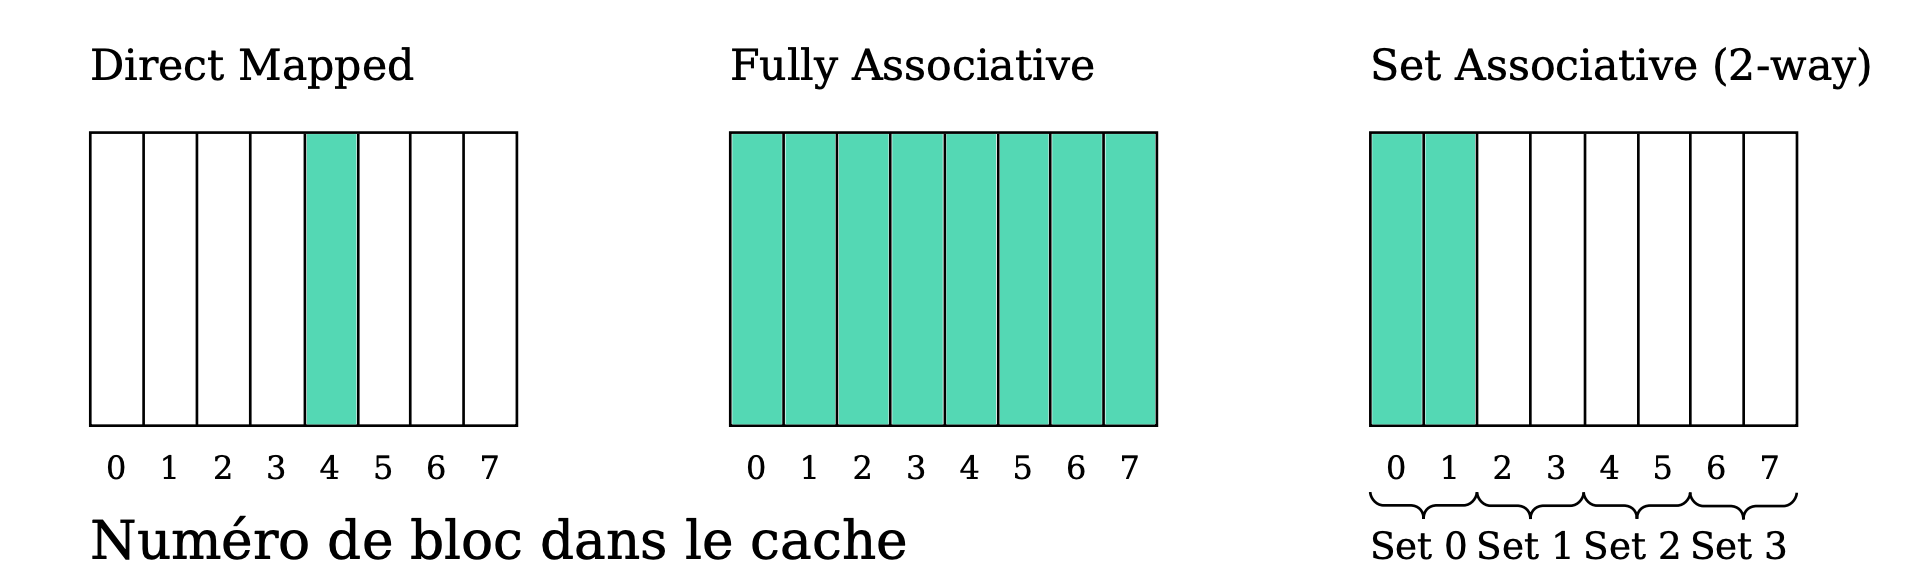
\includegraphics[width=12cm]{images/cache_associativite.png}
    \caption{\label{pic:cache_associativite} En fonction de la politique de remplacement utilisée, une \textit{cache line} sera associée à une ligne du cache différente (source \cite{Meunier2017})}
\end{figure}

\paragraph{Le mappage direct} utilise une fonction simple pour déterminer l'emplacement (index et offset) du cache à utiliser. Une partie des bits est utilisé pour déterminer la ligne à utiliser (\textit{index}) par exemple à l'aide d'une opération modulo. L'autre partie est utilisée pour déterminer le décalage dans cette ligne (\textit{offset}). Cette méthode est très rapide mais peut avoir des performances catastrophiques. Un algorithme faisant des sauts en mémoire d'une certaine taille pourrait n'utiliser qu'une seule ligne du cache, le rendant totalement inefficace.

\paragraph{Le mappage fully associative} remédie à ce problème en permettant à une \textit{cache line} d'être stockée à n'importe quel emplacement dans le cache. Cependant, cette technique à le désavantage d'être très lente. En effet, une \textit{cache line} pouvant se trouver à n'importe quel ligne du cache, il faut toutes les comparer pour vérifier sa présence ou non. Pour faire cette comparaison en parralèle, il faudrait implémenter autant de comparateur que de ligne dans le cache, complexifiant grandement le cache.


\paragraph{Le mappage set associtive } permet de réduire le nombre de comparateur nécessaire en regroupant les lignes du caches potentiellement adressable pour une \textit{cache line} en groupe (\textit{set}). L'exemple de la \autoref{pic:cache_associativite} utilise un cache à 4 set, appelé \textit{4-way associative}. Il ne faut plus que 4 comparateurs pour déterminer si une ligne appartient à un des \textit{set}.


Les mappage par association sont plus lents que le mappage direct, car il faut trouver ou la \textit{cache line} (si présente) se trouve dans un sous ensemble de ligne de cache plus ou moins grand. Ainsi, il nécessite moins de matériel car un seul comparateur est nécessaire pour déterminer la ligne de cache à utiliser. Cependant, le mappage direct peut se trouver  inefficace suivant les acces mémoire réalisés.



\subsubsection{Politique de remplacement}
%%%%%%%%%%%%%%%%%%%%%%%%%%%%%%%%%%%%%%%%%%%%%%%%%%%%%%%%%%%%%%%%%%%
Que ce soit pour le mappage \textit{fully associative} ou \textit{set associative}, une \textit{cache line} peut être stockée à plusieurs ligne du cache. Pour déterminer laquelle choisir pour y placer la \textit{cache line}, différentes stratégies peuvent être utilisée. 

LRU

FIFO




\subsubsection{Stratégie de cache: lecture et écriture}
%%%%%%%%%%%%%%%%%%%%%%%%%%%%%%%%%%%%%%%%%%%%%%%%%%%%%%%%%%%%%%%%%%%









\subsubsection{Propriété d'inclusion}
%%%%%%%%%%%%%%%%%%%%%%%%%%%%%%%%%%%%%%%%%%%%%%%%%%%%%%%%%%%%%%%%%%%
Lorsqu'une donnée est chargé depuis la mémoire, le processeur doit la stocker dans le cache qui varie en fonction de la propriété d'inclusion du processeur pouvant être inclusive ou exclusive ou non-inclusive (voir \autoref{pic:cacheinclusionpolicy}).

Un cache est dit inclusif, si lorsqu'une donnée se trouve à un niveau de la hiérarchie, tous les caches des niveaux supérieur contiennent eux aussi une copie de la donnée (voir \autoref{pic:InclusivePolicy}). Cette politique d'inclusion a un désavantage lorsqu'elle est utilisée sur des système multi-coeurs. En effet, lorsqu'une donnée doit être retiré d'un niveau de cache, le processeur doit aussi l'enlever des niveaux de caches inférieurs. 
Un cache non-inclusif permet qu'une ligne du cache de niveau 1 ne soit pas forcément dans le cache de niveau 2. Cela permet d'augmenter la capacité de la hiérarchie de cache. Les processeurs récents implémente les deux politiques d'inclusion. Le processeur Intel Sandy Bridge a un cache L3 inclusif tandis que les cache L1 et L2 sont non-inclusif.

Pour une politique d'exclusion, une donnée qui se trouve à un niveau du cache, ne peut pas se trouver dans un autre niveau de cache au même moment (voir \autoref{fig:ExclusivePolicy}). L'avantage des caches exclusif est leur capacité de stocker plus de données car une ligne de cache ne se trouve jamais à deux endroits à la fois de la hiérarchie de cache. Cependant, lors d'un \textit{hit} dans le cache L2, le processeur doit échanger la ligne entre les deux niveau de cache L1 et L2, plus long qu'une simple copie.



\begin{figure}
    \centering
    \begin{subfigure}[b]{0.45\linewidth}
        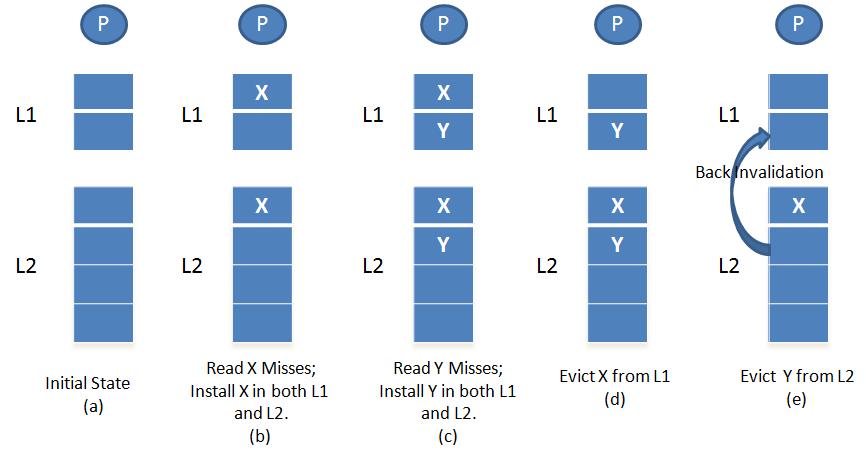
\includegraphics[width=\linewidth]{images/InclusivePolicy.png}
        \caption{Inclusive}
        \label{pic:InclusivePolicy}
    \end{subfigure}
    ~ %add desired spacing between images, e. g. ~, \quad, \qquad, \hfill etc. 
      %(or a blank line to force the subfigure onto a new line)
    \begin{subfigure}[b]{0.45\linewidth}
        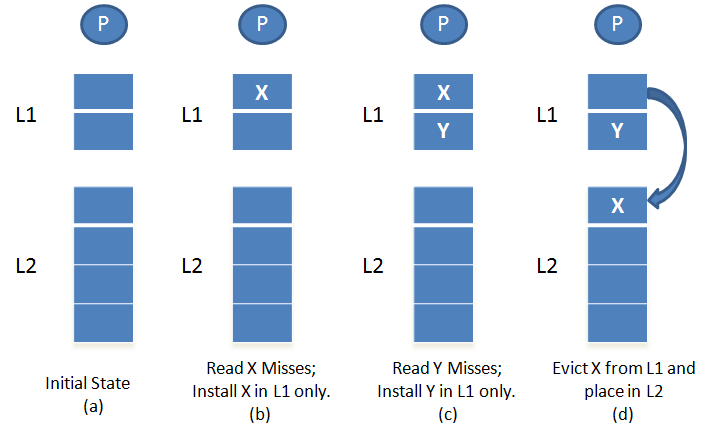
\includegraphics[width=0.85\linewidth]{images/ExclusivePolicy.png}
        \caption{Exclusive}
        \label{pic:ExclusivePolicy}
    \end{subfigure}
    \caption{Exemple de deux propriétés d'inclusion de la hiérarchie de cache (source \cite{wikipedia_2019}). }\label{fig:cacheinclusionpolicy}
\end{figure}





\subsubsection{Stratégie de remplacement}
%%%%%%%%%%%%%%%%%%%%%%%%%%%%%%%%%%%%%%%%%%%%%%%%%%%%%%%%%%%%%%%%%%%







\subsubsection{Cohérence de cache}
%%%%%%%%%%%%%%%%%%%%%%%%%%%%%%%%%%%%%%%%%%%%%%%%%%%%%%%%%%%%%%%%%%%
L'utilisation de cache commun entre différents coeurs d'un même processeur apporte une grande complexité pour gérer la cohérence des données. En effet, une même donnée peut se retrouver dans des cache privé (L1 et L2) de deux coeurs différents. Il faut alors employer des techniques de gestion de cohérence pour assurer la validité des calculs. La gestion de la cohérence d'un processeur à un seul coeur est plus simple, bien qu'elle doive tout de même être implémenté. Les opérations d'entrée-sortie peuvent affecter des données en mémoire qui se trouve aussi dans les caches. Un protocole de cohérence doit garantir trois points. Le premier est de partager le changement d'une valeur à tous les coeurs d'un processeur pour que l'ordre des opérations affecté à une valeur soit vu dans le même ordre par tous les coeurs/processeurs. Le deuxième point est d'assurer que le résultat ne dépende que de l'ordre des instructions du programme assembleur et non de l'ordre de leur exécution par les différents coeurs. Enfin, le protocole doit assurer à un coeur qui lit une donnée que sa valeur est bien la dernières qui a été écrite (par un autre coeur ou autre processeur). 



\subsection{Implémentation}
%%%%%%%%%%%%%%%%%%%%%%%%%%%%%%%%%%%%%%%%%%%%%%%%%%%%%%%%%%%%%%%%%%%

\subsection{Programmation}
%%%%%%%%%%%%%%%%%%%%%%%%%%%%%%%%%%%%%%%%%%%%%%%%%%%%%%%%%%%%%%%%%%%

\subsection{Discussion et conclusion}
%%%%%%%%%%%%%%%%%%%%%%%%%%%%%%%%%%%%%%%%%%%%%%%%%%%%%%%%%%%%%%%%%%%

